\documentclass{article}
%---------------------------
\usepackage{graphicx}
\usepackage{indentfirst}
\usepackage[portrait, margin=1in]{geometry}
\usepackage{setspace}
\usepackage{lipsum}
\usepackage{enumitem}
\setlist[enumerate]{itemsep=0mm}
\usepackage{amsmath,amssymb,amsthm}
\usepackage{multicol,multirow}
\usepackage[nottoc]{tocbibind}
\usepackage[titles]{tocloft}
\usepackage{tikz}
\usepackage{etoolbox}
\usepackage{subcaption}

\usetikzlibrary{shapes.geometric}
\usetikzlibrary{positioning}
\renewcommand{\cftsecleader}{\cftdotfill{\cftdotsep}}
\newcommand{\figref}[1]{Figure~\ref{#1}}
%---------------------------
\newtheorem{theorem}{Theorem}
\newtheorem{lemma}{Lemma}
\newtheorem{corollary}{Corollary}
\newtheorem{definition}{Definition}

\title{CRUST}
\author{David Skocic}
\date{\today}

\begin{document}

\maketitle

\doublespacing
%---------------------------
\vspace{1.5in}
\begin{center}
	\large MTH 496H - Honors Senior Project \\
	\large Fall Semester 2025 \\
	\large Advisor: Dr. Gregory Lupton \\
	\large Cleveland State University \\
	\large Department of Mathematics \& Statistics \\
\end{center}
\vspace{1in}
%---------------------------
\newpage

\tableofcontents
\newpage

\begin{abstract}
	...
\end{abstract}

\newpage

\section{Introduction and Background}

Describe the analysis of algorithms

Define curve reconstruction

give examples why connecting points to the nearest neighbor isn't good

Maybe define "general position"

The crust method of curve reconstruction builds on a few basic geometric tools that are used constantly in discrete geometry in a wide degree of applications. The following sections introduce these tools and prove numerous important and interesting results about them.



\section{Convex Hulls}
The first applicable geometrical tool of interest is the convex hull. A convex hull is used to take a set of points and make a convex shape out of them. It is easy to imagine that there are all sorts of ways to contain every point in a given set $S$ with some sort of convex polygon. You could, for example, draw a square so large that it contains every point in $S$, but an arbitrarily large shape is not very useful. A convex hull  fixes this problem, and adheres to the following definition:
\begin{definition}
	\textbf{(Convex Hull)} For a given set of points $S$, the convex hull is the smallest shape that contains every point in $S$.
\end{definition}

Imagining such a shape for a given set of points is easy. To generate the convex hull for a set of points, imagine the points are nails in a wall. Start by tying a string to a nail at some extrema, say, the leftmost nail on the wall, and holding the string left of that. Then, rotate it all the way around all the other nails until it touches the first one again. This shape the string takes on is the convex hull.

INSERT FIGURE SHOWING THIS IDEA, SHOWING A BIG SQUARE AROUND THE POINTS, AND SHOWING THE FULL CONVEX HULL

The convex hull is a convenient tool because it has a clear definition and because convex shapes tend to be simple to work with. Also, it can serve as a starting point in an algorithm that starts with an unlabeled set of points like the crust. Taking the convex hull at least gives us a place to start connecting our points, even if its usefulness may not initially be clear.

Fortunately, lots of time has been spent finding optimal algorithms for computing the convex hull of a set of points. Here, computing the convex hull really means to find which points from $S$ are vertices of the hull. This can be done in a variety of ways. One being a sort of inductive method that starts with 3 points, then add one at a time from the set, removing points that end up making the shape nonconvex. Another algorithm behaves very similarly to the string wrapping algorithm. While these algorithms are both intuitive, they are not asymptotically optimal.

There also exist multiple algorithms that are asymptotically optimal, with time complexity \textit{O(nlogn)}. From these I will choose my favorite, which uses a divide and conquer approach. I choose this method because of its satisfying recursive nature, and because it is the algorithm that most easily extends to a third dimension.

\textit{this algorithm comes from O'Rourke}
To begin, order the points by their x-coordinate. Next, separate the points into two groups of (approximately) equal size. Now repeat this for both of the new groups, and again for the groups they create until all groups have 1 or 2 points. Now the convex hull is trivial, just a line connecting any two points. The magic of the algorithm comes when bringing the groups back together. \textbf{finish this}

\textit{remember to talk about the actual time complexity of this algorithm versus time complexity of the others mentioned}

\section{Triangulations}
Triangulations are a key tool in the process of curve reconstruction. Specifically, a type of triangulation called a Delaunay triangulation is used to construct the crust of a given set of points. Before diving into Delaunay triangulations and some interesting results that follow, we first explore an easier problem, the triangulation of a polygon, and build up to Delaunay triangulations from there.

\subsection{Triangulations of Polygons}

To begin, we must first define a triangulation of a polygon. \begin{definition}
	\textbf{Triangulation of a Polygon in two dimensions} A decomposition of a polygon into triangles by a maximal set of non-intersecting diagonals.
\end{definition}

In simpler terms, a triangulation breaks a polygon into triangular pieces by drawing segments between its vertices so that no two segments intersect. The term 'maximal set' is used in the definition to ensure that there is no vertex of the polygon on the edge of any triangle.

As an example, let's look at an easy case: a convex octagon. It is easy to pick out a way to triangulate this shape: just start at one vertex and draw lines to every other vertex as shown in \figref{fig_example_triangulations}. It is easy to see how this technique can extend to any convex n-gon to create a triangulation with n-2 triangles. Something of note is that there can be more than one way to triangulate a polygon, with another example shown in \figref{fig_example_triangulations}. Is it possible that some triangulations are better than others? The fact that there is a section dedicated to a specific type, the Delaunay triangulation, should be a clue here, and the reason why is explored in that section.

\begin{figure}
\[
    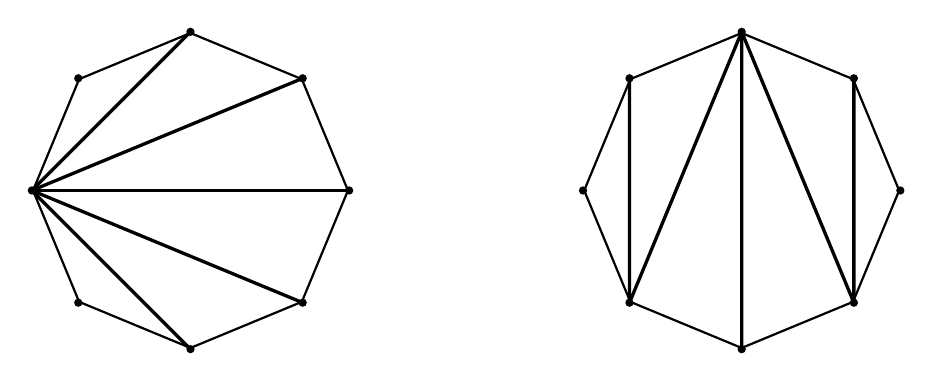
\begin{tikzpicture}
      % regular octagon as a node; change minimum size to scale
      \node[
        draw,
        thick,
        regular polygon,
        regular polygon sides=8,
        minimum size=4cm,    % controls overall size
        rotate=22.5          % optional: rotate so a side is horizontal
      ] (oct1) at (-3,0) {};
    
        % regular octagon as a node; change minimum size to scale
      \node[
        draw,
        thick,
        regular polygon,
        regular polygon sides=8,
        minimum size=4cm,    % controls overall size
        rotate=22.5          % optional: rotate so a side is horizontal
      ] (oct2) at (4,0) {};
      
      \foreach \i in {1,...,8}{
        \fill (oct1.corner \i) circle (1.5pt);
        \fill (oct2.corner \i) circle (1.5pt);
      }
      \foreach \i in {1,5,6,7,8}{
        \draw[black, very thick] (oct1.corner 3) -- (oct1.corner \i);
      }
      \draw[black, very thick] (oct2.corner 4) -- (oct2.corner 2);
      \draw[black, very thick] (oct2.corner 4) -- (oct2.corner 1);
      \draw[black, very thick] (oct2.corner 1) -- (oct2.corner 5);
      \draw[black, very thick] (oct2.corner 1) -- (oct2.corner 6);
      \draw[black, very thick] (oct2.corner 8) -- (oct2.corner 6);

    
    \end{tikzpicture}
\]
\caption{Two example triangulations of a regular octagon.} \label{fig_example_triangulations}
\end{figure}

A more interesting problem arises when you try to triangulate a shape that is nonconvex. Is this even possible for \textit{any} polygon? If it is, is there an algorithmic way that works to triangulate any polygon? Will there always be the same number of triangles? The following theorems dive deeper into these questions.

\begin{theorem}All polygons can be triangulated\end{theorem}

\begin{proof}  %This proof comes from computational geometry by springer
	This is an inductive proof with the base case being a polygon with 3 vertices. This base case is trivial because a triangle need not be broken down into more triangular pieces. Now, the assumption that any polygon with $m$ or fewer vertices can be triangulated and our goal is to show that that a polygon with $n$ vertices with $n = m+1 > 3$ can be triangulated.

	I will begin by showing that a diagonal exists in the polygon, $P$, formed by $n$ vertices. Take some vertex $v$ from $P$ and label the vertices neighboring it $u$ and $w$. If $u$ and $w$ are connected and do not intersect with any edges of $P$, then a diagonal exists. Otherwise, there exists one ore more vertices of $P$ that are inside triangle $uvw$. Now, imagine a line parallel to segment $uw$ that goes through $v$. Let this line sweep toward segment $uw$ until it encounters a vertex of $P$ inside triangle $uvw$ and call this vertex $v'$. The segment $vv'$ must be a diagonal because there are no edges of $P$ between $v$ and $v'$ by the definition of $v'$. So, a diagonal must exist in $P$.

	The existence of this diagonal means that $P$ can be broken into two polygons that share the diagonal as a common edge, with a total of $n+2$ vertices. There are $n+2$ because the $n$ outer edges of the polygon remain part of either new polygon, and the diagonal contributes one edge to each of the newly created polygon, adding two edges. Since each new polygon must have at least 3 vertices, the other must have at most $n-1 = m$ vertices. By the inductive hypothesis, each of these new polygons may be triangulated.

	
\newcommand{\nextindex}[3]{%
  % #1 = current index
  % #2 = maximum index
  % #3 = name of variable to store result
  \pgfmathtruncatemacro{\temp}{#1+1}%
  \ifnum\temp>#2
    \pgfmathtruncatemacro{#3}{1}%
  \else
    \pgfmathtruncatemacro{#3}{\temp}%
  \fi
}

\begin{figure}
\[
\begin{tikzpicture}[scale=1]
  \coordinate (P1) at (0,0);
  \coordinate (P2) at (2,1);
  \coordinate (P3) at (4,0.5);
  \coordinate (P4) at (3,2);
  \coordinate (P5) at (4,3.5);
  \coordinate (P6) at (2,4);
  \coordinate (P7) at (0.5,3);

  \foreach \i in {1,...,7} {
    \nextindex{\i}{7}{\next}
    \draw[thick] (P\i) -- (P\next);
    \fill (P\i) circle (1.5pt);
  }
  \node[font=\scriptsize, above right] at (P1) {v};
  \node[font=\scriptsize, above right] at (P2) {w};
  \node[font=\scriptsize, above left] at (P7) {u};

  \draw[thin]
    (P2) -- (P7);
  
\end{tikzpicture}
\hspace{3cm}
\begin{tikzpicture}[scale=1]
  % --- Define 7 vertices of a nonconvex heptagon ---
  % (Change numbers as you like)
  \coordinate (P1) at (0,0);
  \coordinate (P2) at (2,1);
  \coordinate (P3) at (4,1);
  \coordinate (P4) at (.75,1.75);
  \coordinate (P5) at (4,3.5);
  \coordinate (P6) at (2,4);
  \coordinate (P7) at (0.5,3);

  \foreach \i in {1,...,7} {
    \nextindex{\i}{7}{\next}
    \draw[thick] (P\i) -- (P\next);
    \fill (P\i) circle (1.5pt);
  }
  \node[font=\scriptsize, below] at (P1) {v};
  \node[font=\scriptsize, below right] at (P2) {w};
  \node[font=\scriptsize, above left] at (P7) {u};
  \node[font=\scriptsize, below right] at (P4) {v'};
  
  \draw[dashed]
    (P2) -- (P7);
  \draw[thin]
    (P1) -- (P4);
  
\end{tikzpicture}
\]
\caption{The two cases when trying to draw a diagonal between two points around a starting point.} \label{fig_diagonal_creation}
\end{figure}
\end{proof}

In the process of proving that it is always possible to triangulate any polygon, we have also generated a simple algorithm to triangulate any polygon. If we begin the same way as the proof, drawing a diagonal between some pair of vertices, two smaller shapes are created. Each of these shapes can undergo the same process and create two more shapes. This can be repeated recursively until all the shapes created by the splits are just triangles, so all the diagonals drawn must constitute a triangulation.
\subsection{Triangulations of a Set of Points}

In the previous section, I showed that any polygon can be triangulated. The method to do this started by drawing a single new edge to form a triangle using two preexisting edges. But what if there are no edges at all, and you just have a set of points? You could construct any number of polygons for a given set of points. To make this algorithmic, we must choose a specific one of these polygons to start to triangulate. To do this, we return to the familiar convex hull.

\begin{definition}
	\textbf{Triangulation of a set of Points} FILL OUT THIS DEFINITION
\end{definition}

After computing the convex hull, our situation appears almost like it did in the previous section, but there are still points inside that are not accounted for. To continue down this path, we sincerely hope that the following theorem is true:

\begin{theorem}
	Any set of points $S$ has a triangulation, $T$, such that \textit{Hull(S)}$ \subset T$. --- notation might not be quite right here, we want the edges of the hull to be a part of the edges of T
\end{theorem}

\begin{proof}

	We follow a similar method to the previous proof, using induction. Again, the base case is a set of 3 points, with the obvious triangulation of a triangle, which is also the convex hull of the points. Our hypothesis is that, assuming that a set of points $S$ of size $n$ has triangulation $T$ with \textit{Hull(S)}$ \subset T$, some $S' \supset S$ of size $n+1$ has triangulation $T'$ with \textit{Hull(S')}$ \subset T'$.

	There are two cases for the new vertex $v$ that belongs to $S'$ but not $S$. Either $v$ is inside \textit{Hull(S)}, or it is outside of it. We will examine each case independently:

	Explain that a point outside will have a new hull with two "new edges", and if these two edges are added to the previous triangulation, we still have a triangulation.

	Explain how a point inside the hull is in a triangle, and hence this triangle can just have each vertex connect to the point inside and maintain a triangulation

	...

\end{proof}

\subsection{Delaunay Triangulations}
Now that we know that we can generate some triangulation for any set of points, we can begin to look at a certain type of triangulation, the Delaunay Triangulation. The Delaunay Triangulation of a set of points has interesting properties and is the primary tool in generating the crust of a given set of points. But before we explore those properties, let us first define it.

\begin{definition}
	A \textbf{Delaunay Triangulation} is the triangulation of a set of points $S$ such that the circumcircle of each triangle only contains the vertices of that triangle, and no other points in $S$
\end{definition}
\begin{figure}
\centering

\begin{subfigure}{0.45\textwidth}
\centering
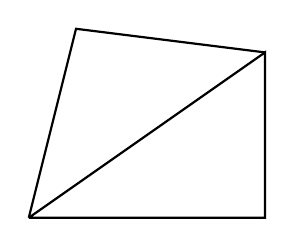
\begin{tikzpicture}[scale=3]
    
    \coordinate (A) at (0,0);
    \coordinate (B) at (1,0);
    \coordinate (C) at (0.2,0.8);
    \coordinate (D) at (1,0.7);
    
    \draw[thick] (A)--(B)--(D)--(A);
    \draw[thick] (A)--(C)--(D);
\end{tikzpicture}
\caption{Non-Delaunay Triangulation}
\end{subfigure}

\hfill

\begin{subfigure}{0.45\textwidth}
\centering
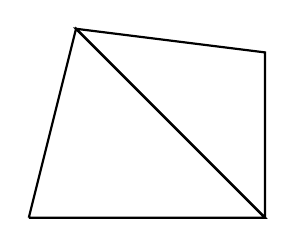
\begin{tikzpicture}[scale=3]    
    % Same points
    \coordinate (A) at (0,0);
    \coordinate (B) at (1,0);
    \coordinate (C) at (0.2,0.8);
    \coordinate (D) at (1,0.7);
    
    % Triangulation (Delaunay: diagonal BC)
    \draw[thick] (A)--(B)--(C)--(A);
    \draw[thick] (B)--(C)--(D)--(B);
\end{tikzpicture}
\caption{Delaunay Triangulation}
\end{subfigure}

\end{figure}


Something you may have noticed in the definition of a Delaunay triangulation is that I claimed that it is \textit{the} triangulation that fits the criteria, not just some triangulation that does. This uniqueness is an important property of Delaunay Triangulations, but it is not at all apparent. Let us show why this is true:

SHOW THAT THE EXISTENCE IS ALSO GUARANTEED

\begin{theorem}
	There is only one Delaunay Triangulation for given set of points $S$.
\end{theorem}
\begin{proof}

\end{proof}

It is of note that if there are four points that are concentric, then there cannot be a triangulation that fits the Delaunay criteria. So, the four points have, in some sense, two valid Delaunay triangulations. We call these triangulations degenerate.

Another interesting property of Delaunay triangulations is that they guarantee that the smallest internal angle of any triangle in the shape is the highest out of all possible triangulations.

\begin{theorem}
	The Delaunay Triangulation has the highest minimum internal angle out of all possible triangulations
\end{theorem}
\begin{proof}

\end{proof}
Effectively, Delaunay triangulations reduce "sliver triangles" which are very long, thin triangles.

talk about angle sequences and transition that into "flipping"

show how you can get from one triangulation to the Delaunay triangulation using progressive steps

dive into talking about the 'flip graph'

show the connection to voronoi diagrams

\section{Voronoi Diagrams}

The third and final tool of interest for the crust is the Voronoi diagram.
Similarly to the other tools introduced so far, the Voronoi diagram takes in a set of points $S$ and returns a structure with useful properties.
But instead of connecting the points in a specific way, the Voronoi diagram consists of lines that pass in between the points to divide the plane into \textit{Voronoi regions}.
Each of these regions contains a single $p\in S$, and is constructed such that any other point is in the region is closer to $p$ than any other point in $S$.
This definition is often much more intuitive than that of the Delaunay triangulation, and lends itself to a wide array of applications.
For instance, to find the nearest post office for any given house on a map, the map could be separated into Voronoi regions where $S$ are the locations of the post offices.
Then, whichever region a house falls into is simply nearest to the corresponding post office.
Voronoi diagrams come up in nature, too;
if many structures began to grow from a starting point at the same rate until they collided, like crystals for example, the area of each crystal would be the Voronoi region of the starting point.

The following is a formal definition of the Voronoi region from Devadoss and O'Rourke.


\begin{definition}[Voronoi Region]
	For a point $p$ in set of points $S$, The Voronoi region of p, Vor(p), is such that
	\[ \mathrm{Vor}(p) = \lbrace x\in \mathbb{R} \hspace{4pt} | \hspace{4pt} ||x-p|| \le ||x-q|| \hspace{4pt} \forall q \in S \rbrace \]
\end{definition}


We can also define Voronoi regions in a different way.
Looking at any other point $q$ in $S$, the perpendicular bisector of $\overline{pq}$ divides the plane into two half-planes, one of which contains $p$, which we will call $H$.
Vor($p$) for this two-point case is just the half-plane described above, and it obviously is for any pair of points.
Going further and considering a three-point system, there are two half-planes that contain $p$.
Clearly anything not in one or both of the half-planes cannot be in Vor($p$), or conversely, everything in their intersection must be in Vor($p$).
We can extend this idea to the following definition:

\begin{definition}[Voronoi Region (Alternate Definition)]
	Vor($p$) is the intersection of all half-planes that contain $p$.
\end{definition}

The benefit of this definition is that it clarifies a few interesting features of Voronoi regions.
First, we can immediately see that Voronoi regions are convex by ...
This follows from the INSERT THEOREM FROM CONVEX HULL SECTION.
This definition is perhaps more indicative of what points in the plane are equidistant to multiple points in $S$: those that lie on the perpendicular bisectors that make up the edges of a Voronoi region.
In fact, the points that are equidistant to multiple points in $S$ are how the Voronoi diagram is defined:

\begin{definition}[Voronoi Diagram]
	The Voronoi diagram of a set of points $S$ is the collection of all points in the plane that are on the boundary of a Voronoi region.
\end{definition}

Or alternatively,
\begin{definition}[Voronoi Diagram (Alternate Definition)]
	The Voronoi diagram of a set of points $S$ is the collection of all points in the plane that are equidistant to at least two points in $S$.
\end{definition}

\begin{figure}
	\centering
	\includegraphics[width=0.4\linewidth]{figures/voronoi_diagram.png}
	\label{fig:voronoi_diagram}
\end{figure}

It follows from this alternate definition that there is always a valid Voronoi diagram, and that there is only one such diagram for any $S$.
This is because any point in the plane has an assignment: either it is equidistant to multiple points in $S$ or it isn't.
Fortunately, this means there is much less work to do compared to the section on the Delaunay triangluation.

Let's turn our attention towards the edges and vertices of the Voronoi diagram.
By its definition, any point in the Voronoi diagram is equidistant to at least two points in $S$.
I will give a formal definition of Voronoi edges and vertices, but a visual example like \figref{fig:voronoi_diagram} is much easier to understand.
The Voronoi edges are the straight lines in a Voronoi diagram and the vertices are the points where these edges meet.

A sufficient definition of the Voronoi edges is the set of points in the plane that are equidistant to exactly two points in $S$, and Voronoi vertices are the points in the plane equidistant to at least three points in $S$.
In other words, you could draw a circle centered around any Voronoi vertex that connects three points in $S$.
And there must exist no point $q\in S$ inside this circle, otherwise the vertex wouldn't belong to the Voronoi diagram because it would be closer to $q$ than all other points in $S$.
So if we connect these three points, we recover exactly the empty circle property that we used to define the Delaunay triangulation!

This turns out to be more than an interesting coincidence; it's actually a direct link between the Delaunay triangulation and the Voronoi diagram.
If the Voronoi vertices are the centers of all circles that bound three points which have triangles obeying the empty circle property, then if we know all the Voronoi vertices, we also know which points to connect to create the Delaunay triangulation.
This goes the other way, too.
If we have the Delaunay triangulation, taking the circumcircle of each triangle returns all Voronoi vertices.
And since the Voronoi vertices are where Voronoi edges meet, the centers of each circumcircle must be connected to form the Voronoi edges.

And from here we obtain our algorithm to compute the Voronoi diagram:

\begin{algorithm}
\end{algorithm}


\section{The Crust}
It is finally time to put the geometric tools that this paper has focused on so heavily to use to define the crust of a set of points. As a reminder, the crust is a method of curve reconstruction introduced by \cite{AMENTA1998125}, which is where all the definitions come from in this section. It begins with a set of points taken from a smooth curve with the assumption that they are close enough together to be reconstruction. This "close enough" condition is defined later in the section on sampling. The crust has the following simple definition:

\begin{definition}[The Crust]
	Let $S$ be a set of finite points in the plane, and let $V$ be the vertices of the Voronoi diagram of $S$. Next let $S'=S \cup V$ and consider the Delaunay Triangulation of $S'$. Any edge of the Delaunay triangulation of $S'$ that connects two points in $S$ is an edge of the crust.
\end{definition}

INSERT A FIGURE IN THIS SECTION WITH AN EXAMPLE SIMILAR TO PAGE 3 OF THE PAPER

This is a fairly simple definition, and yet I claim that it can often successfully reconstruct a curve from a set of points in the plane. Before formally proving that this is true for a certain sampling condition, I will provide some intuition on why this is the case. To do this, I will give an alternate but equivalent definition of the crust that uses the familiar empty circle property:

\begin{definition}[Alternate Definition of The Crust]
	Let $S$ be a set of finite points in the plane, and let $V$ be the vertices of the Voronoi diagram of $S$. An edge connecting two points in $S$ belongs to the crust of $S$ if there is a disk containing no other points in $S \cup V$.
\end{definition}

It also helps to note that Voronoi vertices are at the corners of regions of proximity, so they are closer to the points from $S$ in adjacent Voronoi regions than to any other points in $S$. This means that points that obey the alternative definition are connected with those in nearby proximity regions, not simply points that are closest together.

Also, looking at a few examples of Voronoi diagrams of many points, one can see that the diagram draws a line approximately through the middle of the shape that they create. This line is called the medial axis and will be explained further in the next section, but the idea is that the Voronoi edges trace out a line through the middle of a shape, then the empty circle properly serves to prevent lines from being drawn through this center line of the shape.


\section{The Medial Axis}
This section begins to lay the foundation to prove that the crust is a valid method to reconstruct a curve, with a few interesting results along the way. First, I will define the medial axis, but intuitively it can be thought of as a Voronoi diagram for an infinite set of points \cite{AMENTA1998125}.


\section{Sampling}
\subsection{Local Feature Size}

\input{source/examples.tex}


\newpage
\nocite{*}
\bibliographystyle{apalike}
\bibliography{CRUST}
\end{document}
